\documentclass[12pt]{article}
\usepackage[margin=0.8in]{geometry}
\usepackage{blindtext}
\usepackage{multicol}
\usepackage{amsmath}
\usepackage[load={physical}]{SIunits}
\usepackage{graphicx}
\usepackage{float}
\usepackage{hyperref}

\usepackage[font=footnotesize]{caption}

\newcommand{\po}{{}^{210}\text{Po}}

\setlength{\columnsep}{1cm}

\title{Alpha particle spectroscopy}


\author{Will Bodron \\ Department of Physics \& Astronomy \\ University of Kentucky}

\begin{document}

\maketitle

\begin{abstract}
    \textit{The energy of alpha particles emitted by $\po$ is measured using a silicon surface barrier detector. By increasing the density of air between the source and the detector, the effective range of 5.3 $\mega \electronvolt$ alpha particles and the energy dependence of the rate of energy loss can be measured.}
\end{abstract}

\begin{multicols}{2}

    \section{Introduction}
    % Scope and significance
    \paragraph{} Monoenergetic alpha particles are emitted via nuclear decay from $\po$ atoms. By varying the density of an air absorber and measuring the energy of $\alpha$-particles incident on a silicon barrier detector, we can determine the energy dependence of the rate of energy loss for $\alpha$-particles. \cite{kovash} The `curve' generated by the relationship between peak energy and air density is known as a Bragg curve, and is commonly used medicine to determine (and even leverage) the depth at which energy loss occurs. In radiation therapy for cancer, particular Bragg Peaks are used to minimally invasively target cites underneath tissue by focusing the depth of greatest energy loss on the tumor \cite{brookhaven}. Most Bragg curves spike strongly just before their stopping point. This has the effect of leaving little damage to surrounding healthy tissue. It is therefore imperative to be able to measure accurately the rate of energy loss as a function of the thickness of the absorber.
    \paragraph{} We may also use alpha particle spectroscopy to identify which radionuclide they originated from. $\po$ is especially rare, and determining the isotope you may have created by some nuclear process or found in a naturally occurring sample can be done by examining the resulting energy curves obtained via alpha spectroscopy.

    $\po$ has 84 protons, an atomic mass of $209.98 u$, and a half-life of $138.376 d$ \cite{table}. Polonium-210 almost always undergoes alpha decay, resulting in ${}^{206}Pb$.
    \begin{equation}
        \po \rightarrow \alpha + {}^{206}Pb
    \end{equation}
    With such a short half-life and predictable nuclear decay pattern, polonium-210 has been studied in depth and has been the subject of controversies such as the assassination of one Alexander V. Litvineko \cite{roessler}.


    \section{Theory}
    
    \paragraph{} We first note that $\alpha$-particles are emitted isotropically from a source \cite{kovash}. Therefore, we determine the solid angle subtended by the detector in order to approximate the total number of particles emitted. Given a distance from the source to the center of a circular detector as $R$ and the diameter of the silicon detector, $d$, we find that the solid angle subtended is:
    \begin{equation}
        \Omega = 2\pi\left(1-\frac{R}{\sqrt{R^2 + \frac{d^2}{4}}}\right)
        \label{solidAngle}
    \end{equation}
    Then, pumping a vacuum between the source and the detector prevents the alpha particles from being stopped by the air absorber. Thus the total number of decays per second can be written as:\footnote{An approximation based on the flat surface area of the detector leads to an over estimate of 9\% of the ratio of particles measured to total emitted.}
    \begin{equation}
        \frac{\text{decays}}{\text{second}} = \frac{N_{detected}\Omega}{4\pi t_{trial}}
    \end{equation}
    Where $t_{trial}$ represents the duration of the detection period. Curies, then, are defined as $1 Ci = 3.7 \times 10^{10}$ decays/second. We will use the MCA spectrum analyzer and the MAESTRO software to collect a spectrum over a duration of 5 minutes, and integrate over all channels to find the number of alpha particles that landed on the detector. \cite{kovash}

    \paragraph{} MCA channels are analogous to detected particle energy and there exists a linear calibration to convert channels to energy values. This calibration can be created using a model 419 pulser, capable of generating pulses similar to those created by the silicon surface detector. By attenuating the height of these regularly generated pulses, we can perform a linear fit to the attenuation-channel data-points. The x-intercept of this fit defines the pedestal channel which represents detected particles of 0 energy. The fit can then be normalized using a single data point. We know the energy of an alpha particle in a vacuum to be 5.3 MeV. Define the energy of the centroid channel for a spectrum obtained at a minimum pressure to be 5.3 MeV. These two data points can be used to interpolate the relationship between MCA channel and energy. \cite{kovash}

    The theoretical value of the energy loss of a projectile is modelled via the particle's dominant loss mechanism, its interaction with atomic electrons. The Bethe-Bloch formula
    \begin{equation}
        -\frac{dE}{dx} = 2\pi r_e^2(m_ec^2)^2Z_p^2N\left(\frac{m_p}{m_e}\right)\left(\frac{B}{E}\right)
        \label{bethebloch}
    \end{equation}
    with $Z_p$ as the particle charge, $N$ as the target density in atoms, and $B$ as the atomic stopping number, calculated as
    $$B = Z_t\ln\left(\frac{4m_eE}{m_pI} - 0.90\right).$$
    The mean ionization energy, $I$, is 32.5 eV for an air absorber, and the value of $Z_t$ is the weighted mean of the values for each of the constituent atoms.
    In order to find rate of energy loss through a medium, we must fill the space between our source and detector with substance of known areal density. The areal density is defined as
    \begin{equation}
        \tau = \rho \times L
        \label{areal}
    \end{equation}
    where $\rho$ is the volume density and $L$ is the linear thickness, and it can be calculated for air at a known temperature and humidity. We can also convert loss rate to units of thickness as an areal density using 
    \begin{equation}
        \frac{dE}{d\tau} = \frac{1}{\rho}\frac{dE}{dx}
        \label{arealConversion}
    \end{equation}
    This derivate will be measured directly by looking at $\Delta E$ and $\Delta \tau$ for every adjacent pairs of data points.
    Finally, the range of a particle of energy $E_0$ can be calculated from the rate of energy loss using 
    
    \begin{equation}
        R(E_0) = \int_0^{E_0} \frac{dE}{-dE/d\tau}
        \label{range}
    \end{equation}

    \section{Experimental Methods}

    A silicon semiconductor detector generates pulses to a preamplifier and in turn an amplifier with pulse heights proportional to the energy of the detected particle. Between the sample and the detector variable absorbers are inserted by controlling the density of air within the experiment chamber. Distances were measured for the approximation of the radioactivity,
    \begin{table}[H]
        \begin{center}
            \begin{tabular}{| c | c | }
                \hline
                Dimension & Length ($\milli\metre$) \\
                \hline
                Detector & $14 \pm 2$ \\
                Source & $54 \pm 2$ \\
                Detector diameter & $13 \pm 0.5$ \\
                \hline
            \end{tabular}
        \end{center}
        \caption{Experimental Setup}
        \label{table:1}
    \end{table}

    To measure the radioactivity of our $\po$ sample, the solid angle subtended by the silicon detector as viewed from the sample was measured to be $s = 81.4\pm7.3$ millisterradians using eq. \ref{solidAngle}. A count of the emissions measured by the silicon detector at the lowest pressure attainable with our vacuum pump (7 torr), over multiple trials to be $R = 26.00 \pm 0.30$ counts per seconds. Therefore, the total decays per second from the (otherwise known as the radioactivity measured in Becquerel), can be calculated as
    \begin{equation}
        R\cdot\frac{4\pi}{s} = 4014.55 \pm 65.63 \becquerel,
    \end{equation}
    or $0.1085 \pm 0.0018 \micro\curie$. The manufacturer sells the samples with radioactivity of $0.1\micro\curie$\footnote{\href{https://www.pasco.com/products/lab-apparatus/atomic-and-nuclear/sn-9085}{Store website}}, citing only one significant digit.
    \begin{figure}[H]
        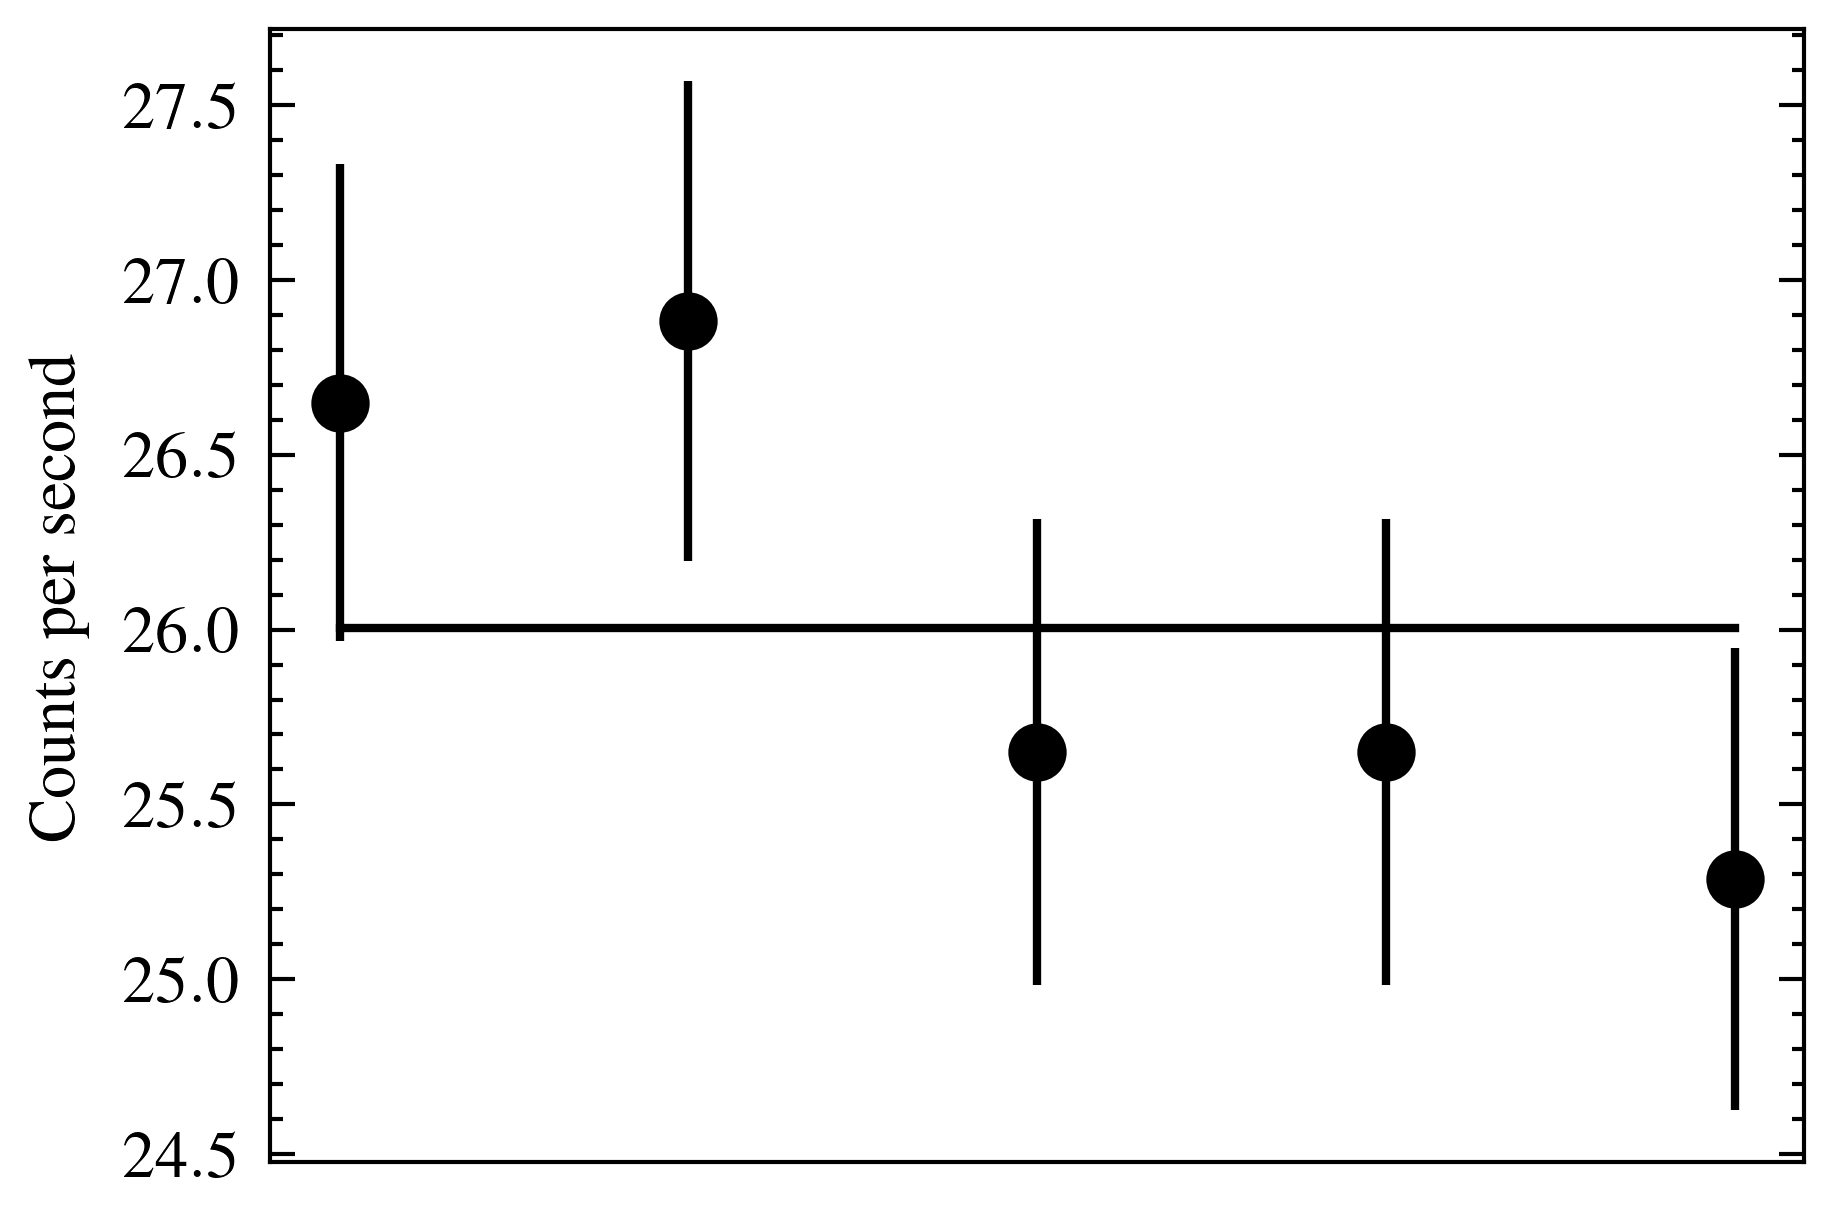
\includegraphics[width=0.45\textwidth]{charts/sample_bq.png}
        \caption{Average $\alpha$'s detected per second in vacuum}
    \end{figure}

    \subsection{MCA Calibration}
    The multi-channel analyzer is a software and hardware pair that creates a histogram of peak heights. Peak heights are binned into channels of arbitrary width, so it is desirable to find a calibration between MCA channels and incident particle energy. This curve may be extrapolated from the energy of two known channels: (a) the channel that contains the peak $5.3 \mega\electronvolt$, the known peak energy for $\alpha$ particles created by $\po$ in vacuum and (b) the channel associated with the notion of having a peak with zero height. To find (b), the pedestal channel, we attenuate the output of a specialized signal generator that regularly creates pulses of similar shape to those created by the silicon surface barrier detector. With this, we can determine the channel associated with a particular attenuation. Repeating the process 5 times, attenuating to the values $0.1, 0.2, 0.25, 0.5,$ and $1$, we receive a relationship that fits well linearly. Therefore, it is safe to assume that the relationship between channels and energy is linear as well.

    \begin{figure}[H]
        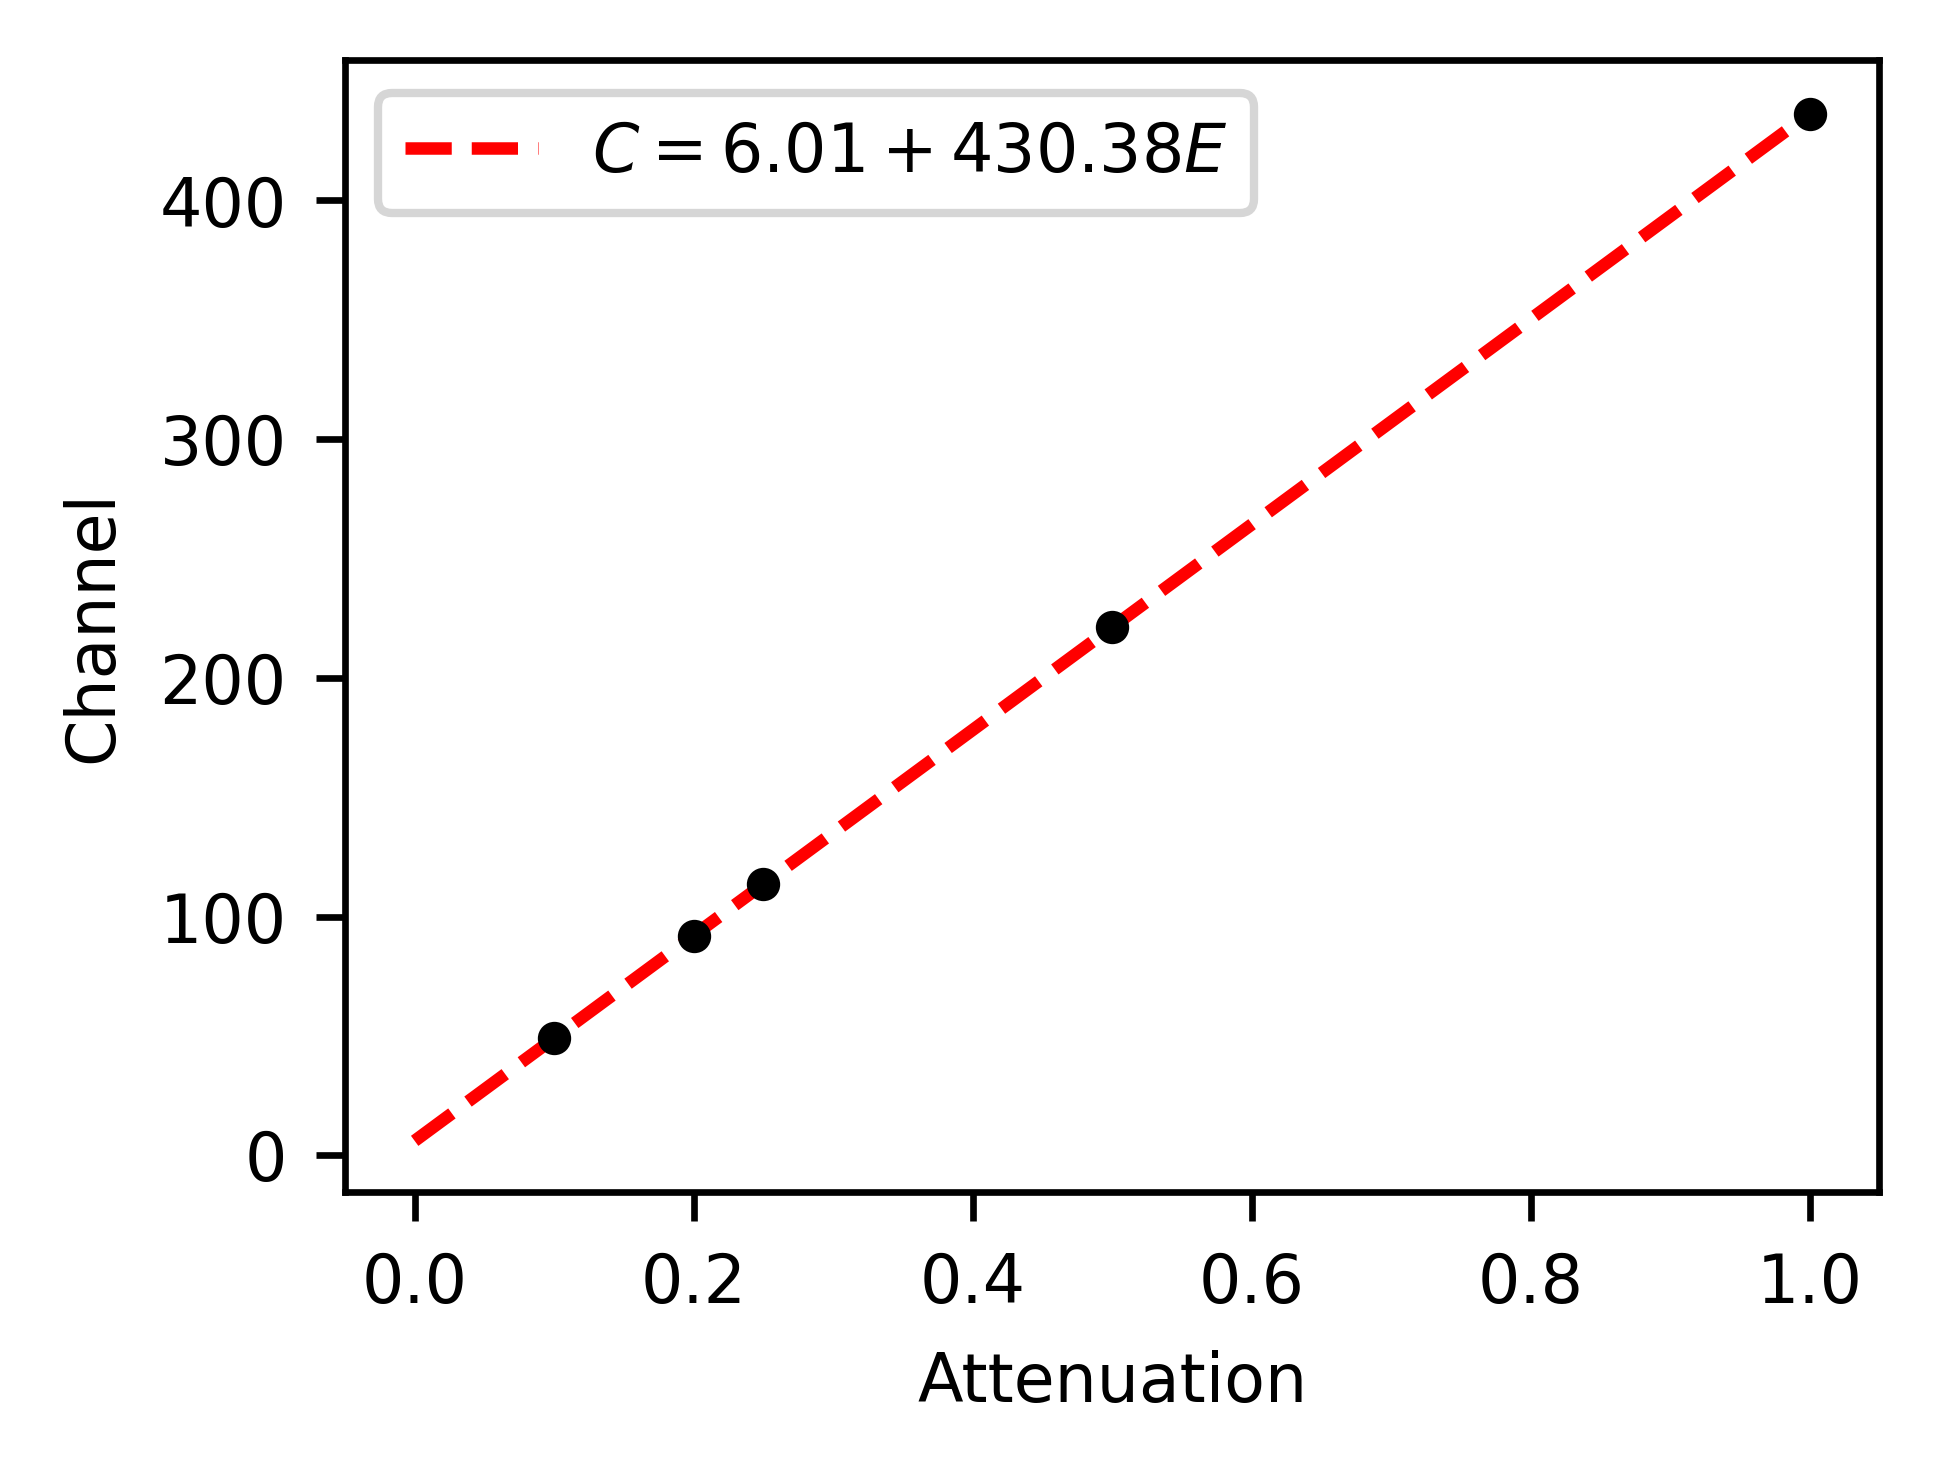
\includegraphics{charts/calibration.png}
        \caption{Identification of pedestal channel}
    \end{figure}

    The $y$ intercept, $6.01\pm 0.006$ represents then the pedestal channel. Now knowing the relationship to be linear and having two datapoints, we use point slope form to represent the calibration between channels and energies:
    \begin{equation}
        E(C) = 5.3 \cdot \frac{C - 6.01}{418.6 - 6.01} = 0.0128(C - 6.01)
        \label{calibration}
    \end{equation}

    \subsection{Centroid Repeatability}
    \label{centroid}
    At this stage in the analysis, I was curious about the repeatability of finding the channel associated with peak energy. Duplicate spectra for a range of pressures were taken and the sample variance for two methods of isolating a peak were compared. Even if the method was systematically wrong, it could be valuable due to the nature of the calibration process. The method I settled on was to convolve a hamming window of width 15 through the spectra and calculate an `$\text{argmax}$.' This method reduced the sample standard deviation by a factor of 2 when compared to using the channel associated with the absolute maximum. From here onward, any channel should be quoted with having $\pm 1$ channel of uncertainty. We note that uncertainty in the peak channel increases with straggling at higher pressure, and that our peaks are broadened by air leaking into the tank. We should also note that the values of the first couple channels were thrown out. They would represents negative energy values according to our calibration and appeared as the absolute maximum before on the spectrum analyzer

    \subsection{Straggling calculation}
    The full width half max of spectra was calculated by splitting the spectra at its maximum, and performing spline interpolation on the inverse of each part. Evaluating each of these inverse interpolations at half the maximum, and taking the difference of the results gets us the FWHM channels, which can then be converted to energy using the calibration curve (eq. \ref{calibration}). The FWHM acts as a measure of ``straggling.''

    \section{Results}

    After collecting spectra from a range of pressures, we convert pressures to areal density, and the collected channel information into related energies. Peaks were found using the method presented in section \ref{centroid}.
    \begin{figure}[H]
        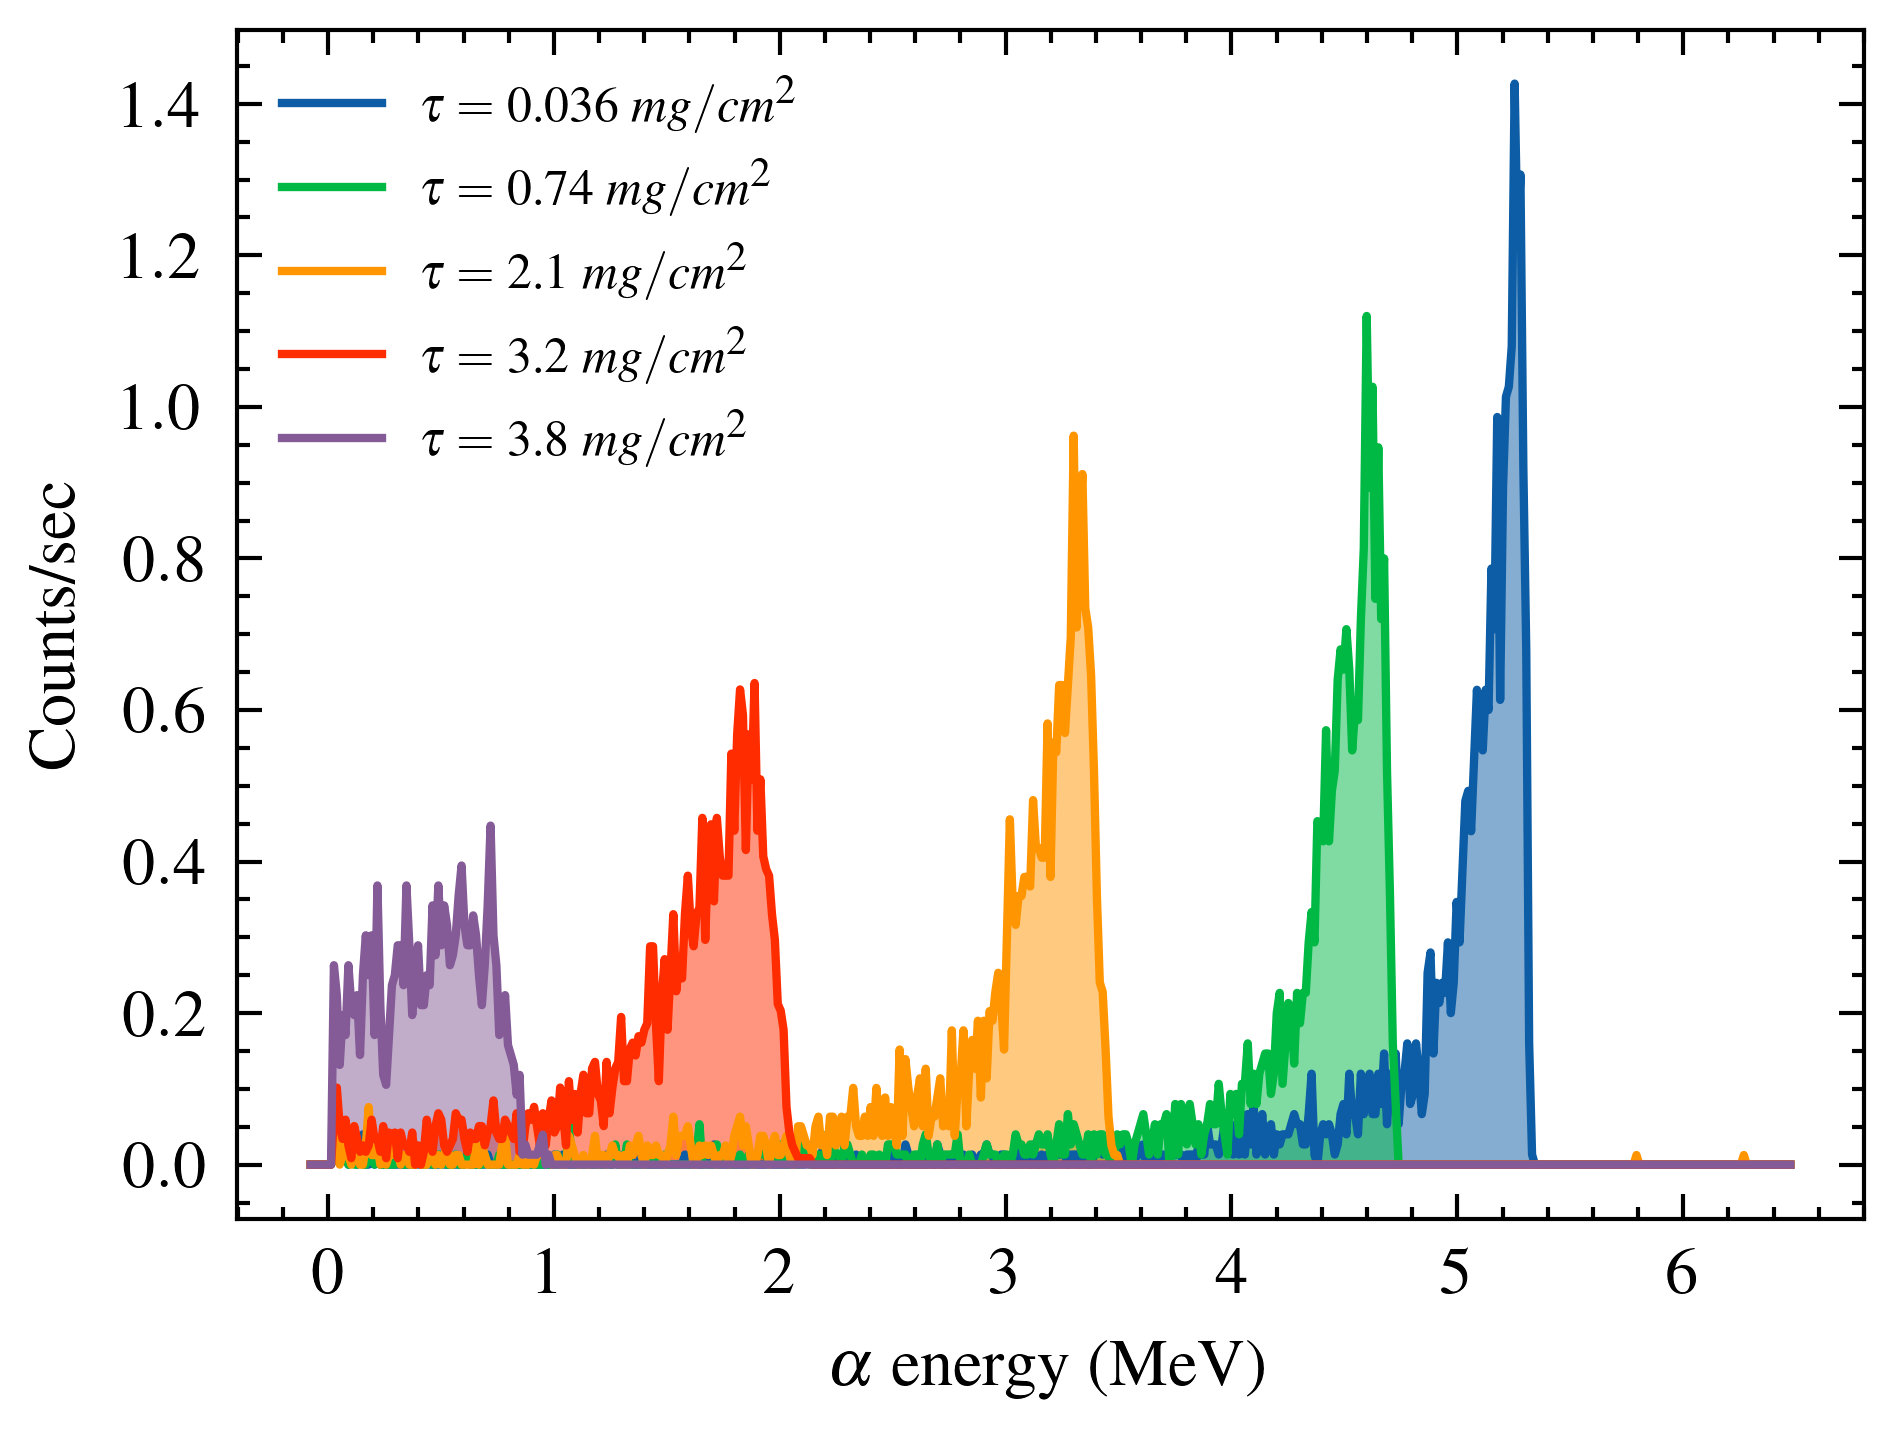
\includegraphics[width=0.45\textwidth]{charts/spectra.png}
        \caption{A sample of $\alpha$ spectra collected from an MCA spectrum analyzer at different pressures}
    \end{figure}
    The energy of peaks is charted as a function of areal density, and extrapolated from the right to find the range of alpha particles. Note that at zero density, the peak energy detected lies at 5.3 $\mega \electronvolt$ as we would expect. The energy of particles is expected to be zero at $4.16 \pm 0.04 \centi \metre$, extrapolated from only the higher densities.
    \begin{figure}[H]
        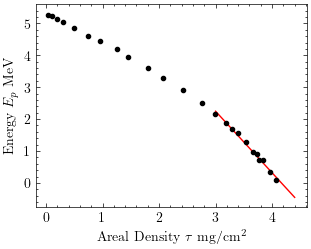
\includegraphics[width=0.45\textwidth]{charts/Energy.png}
        \caption{Areal density v. Energy}
        \label{energy}
    \end{figure}

    A numerical derivate of figure \ref{energy} using medians was performed to acquire $dE_p/d\tau$. The negative is taken to show the energy deposited to the environment and for the convention with the Bethe-Bloch equation \ref{bethebloch}. 

    \begin{figure}[H]
        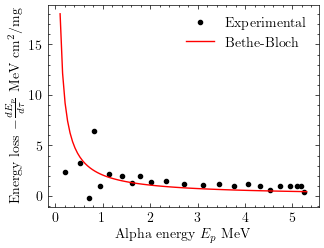
\includegraphics[width=0.45\textwidth]{charts/EnergyLoss.png}
        \caption{Energy v. Rate of energy loss}
        \label{energyloss}
    \end{figure}

    Though the theory works quite well at high alpha energy, the energy loss for the lower energy alphas are subject to greater standard error due to less particles reaching the detector. This is illustrated well on a graph of counts per second against density.

    \begin{figure}[H]
        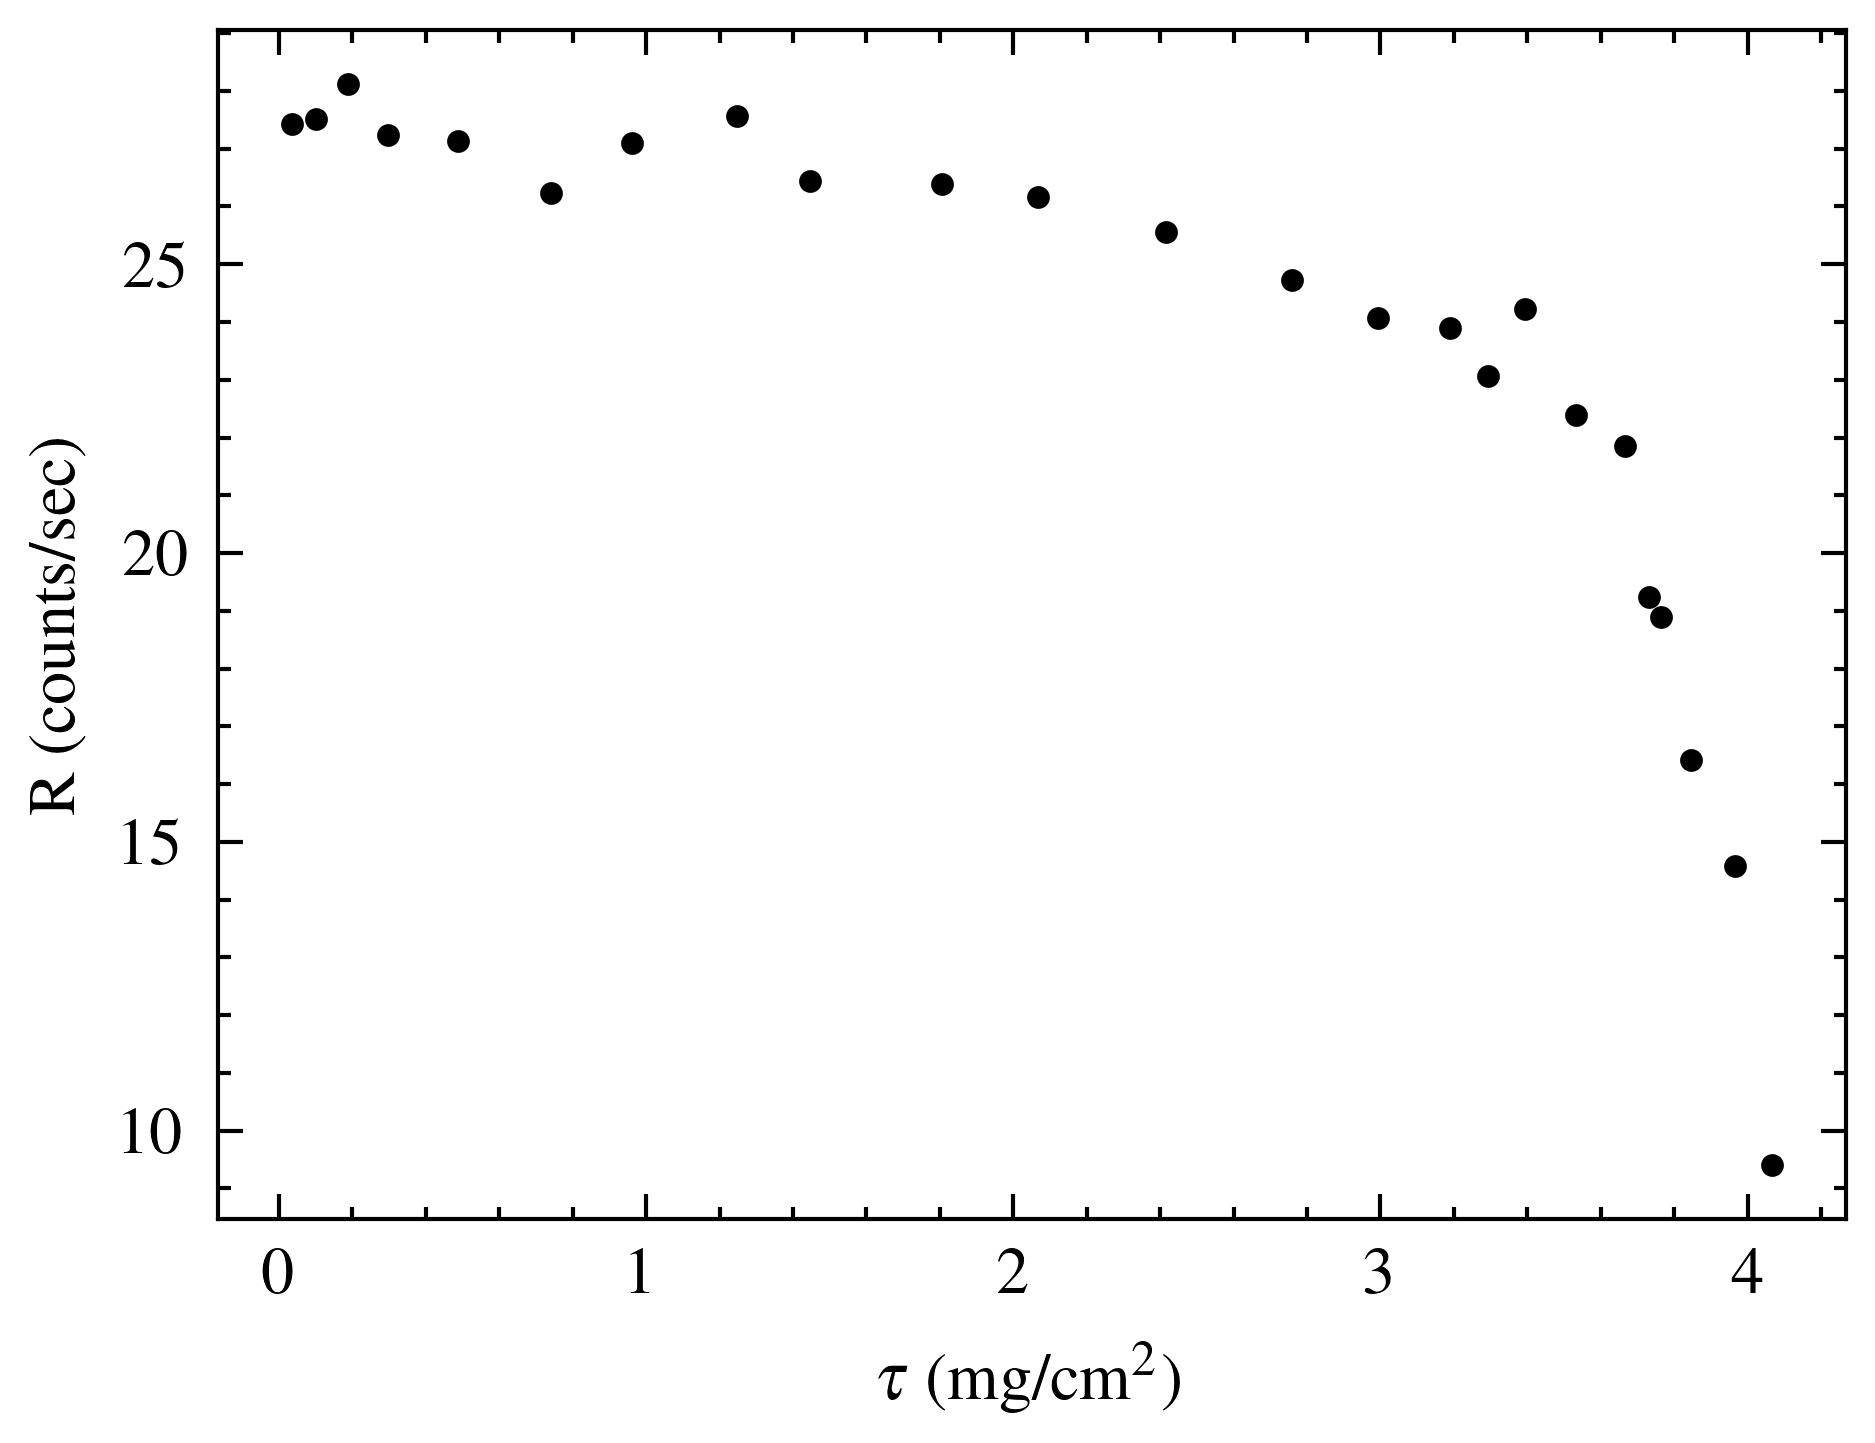
\includegraphics[width=0.45\textwidth]{charts/R.png}
        \caption{As the pressure increases, less alpha particles are able to reach the detector.}
        \label{R}
    \end{figure}

    As particles are subject to greater density absorbers, their energy decreases. At low enough energies, ionization of the absorber begins to effect the trajectory of particles more and more. The total counts per second chart indicates that some or nearly all particles passing through absorbers of areal density from 3.5 to 4 $\milli \gram \per \centi \metre^2$ are stopped before reaching the detector. In a future experiment, the distance between the detector and the source should be reduced from $4\centi \metre$ to $3.5 \centi \metre$.

    Particle straggling occurs when the trajectory of particles affected enough to cause alpha particles to travel longer distances through the medium before reaching the detector. These particles that have traveled less direct routes will land on the detector with lower energy and give a more uniformly distributed spectrum. A metric for this effect can be found in the full width at half max of the peak of the spectrum. 
    
    \begin{figure}[H]
        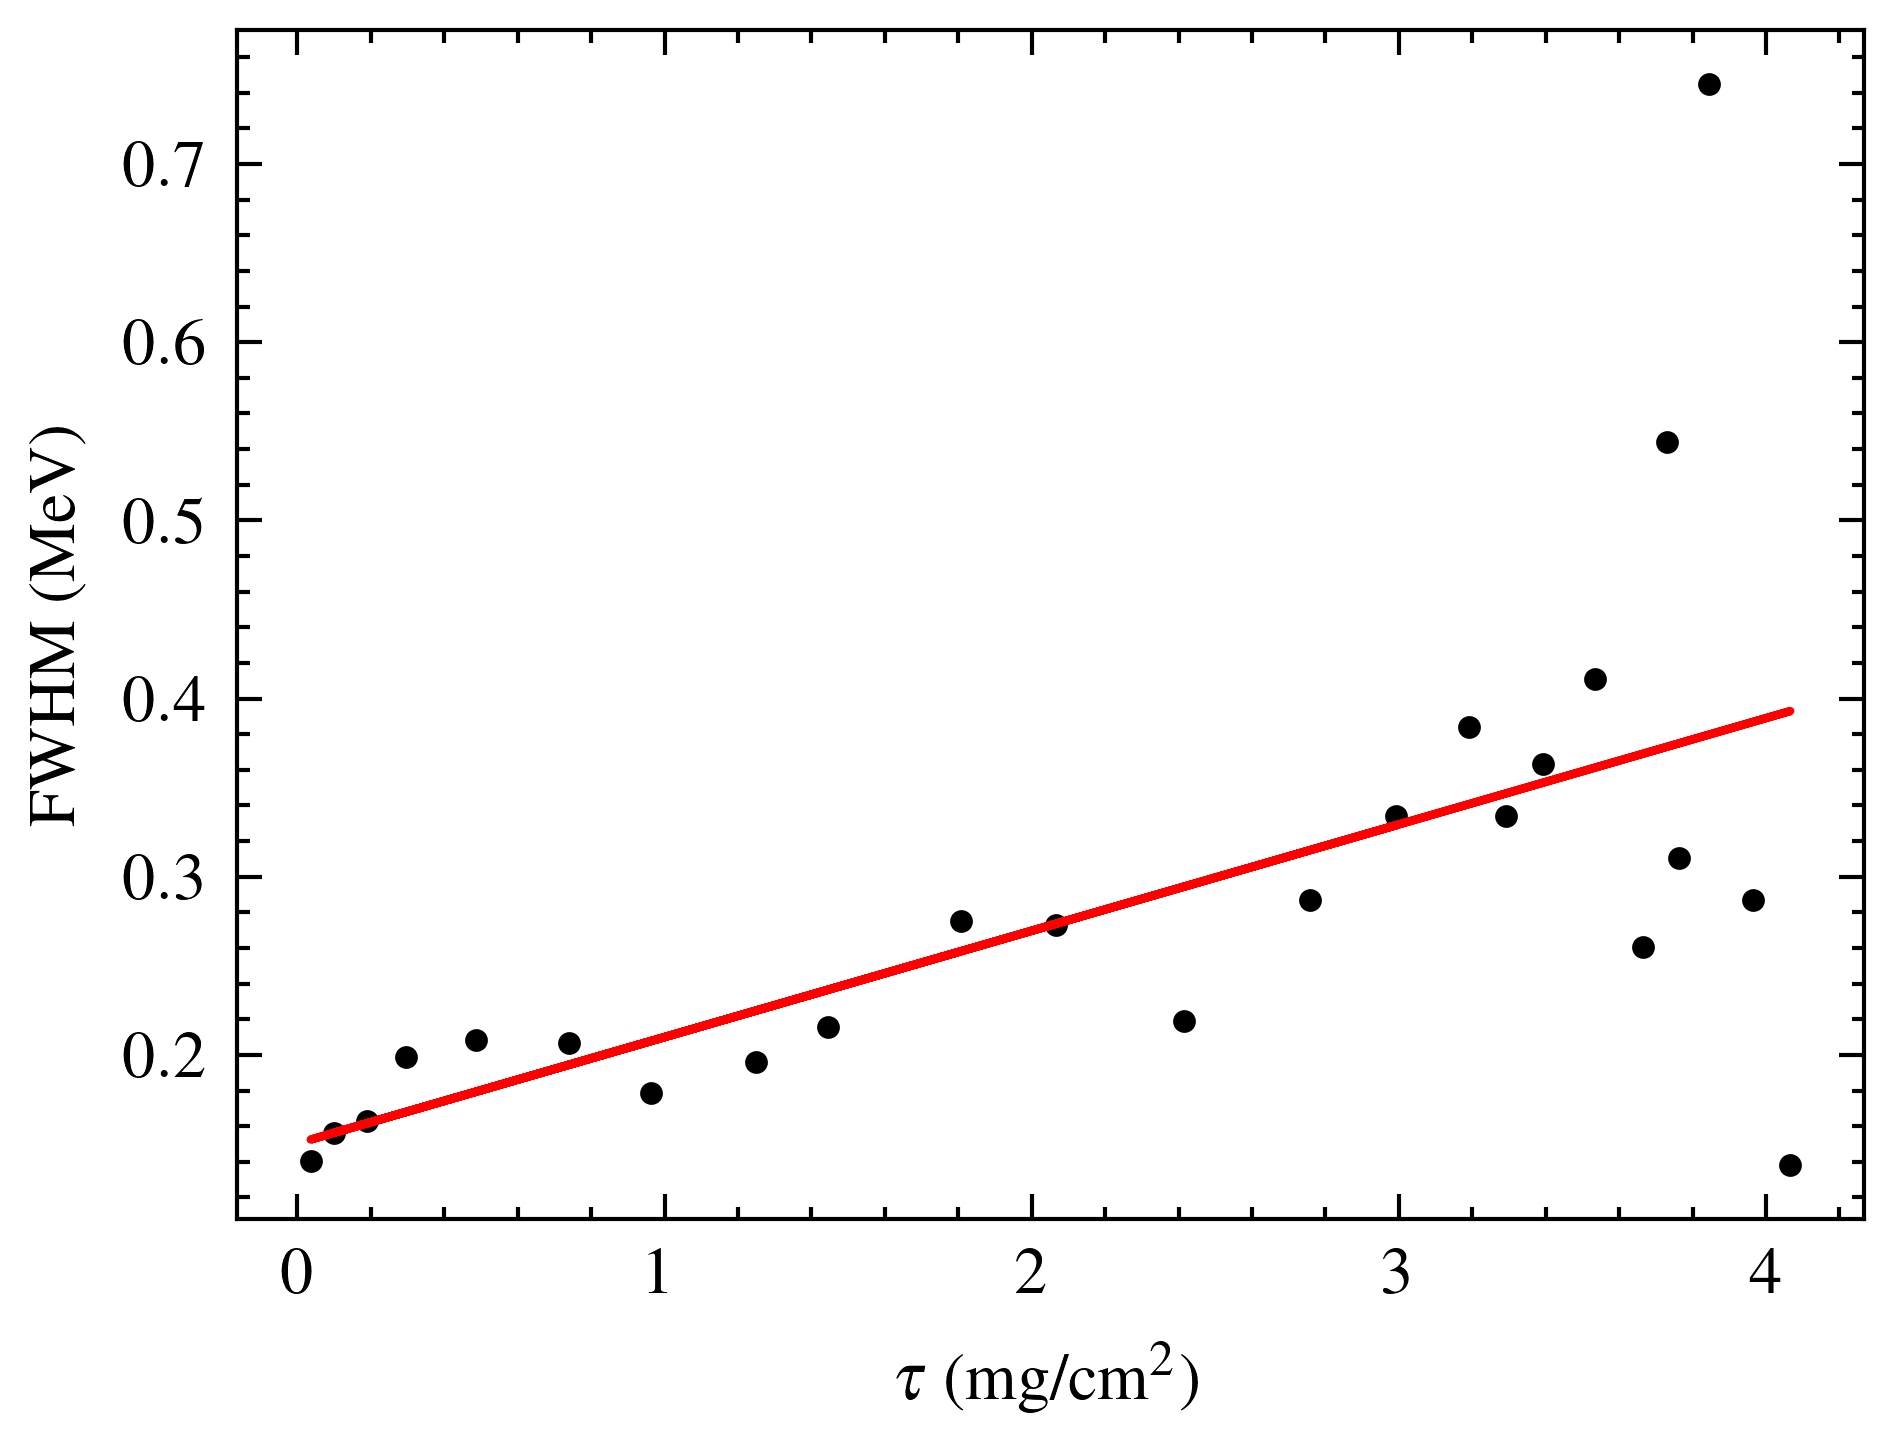
\includegraphics[width=0.45\textwidth]{charts/FWHM.png}
        \caption{Particle Straggling}
        \label{fwhm}
    \end{figure}
    We assert that the principle of straggling is consistent with the upward slope with respect to density. Noting that the energy loss increases more quickly for low energy particles, high energy particles should be able to blast through a low density absorber without being deflected. At a certain turning point, around 1 MeV, the particles will appear to suddenly start taking significantly longer tours, onsetting near the detector. The right side of the FWHM chart shows a decrease again at $\tau = 4 \milli \gram \per \centi \metre^2$. This can be explained with the notion that the FWHM at that point is also a measure of the maximum particle energy, as the peak of the spectrum will contain both 0 and the highest incident particle. The highest likely incident particle in this case may have very low energy, and in our case lies at 0.1 MeV.

    \section{Conclusion}

    \section{Appendix}
    Because of the nature of the data in this experiment, I was afforded the opportunity to create something I would consider very special

    \bibliographystyle{plain}
    \bibliography{refs.bib}
\end{multicols}
\end{document}